\section{Data Generation}\label{sec:data}

\subsection{Single-transistor datasets (Part A)}\label{sec:data:gen}
For each case (NMOS ON, NMOS OFF, PMOS ON, PMOS OFF) one ngspice netlist generates 10,000 samples without any external script: a \texttt{.control} loop draws the sample with \texttt{sunif(0)}, applies it with \texttt{alter} (sources, width), \texttt{altermod} (model parameters) and \texttt{option temp}, runs \texttt{.op}, and appends one CSV row with \texttt{echo}. Every terminal has its own voltage source ($V_d,V_g,V_s,V_b$) and the currents are recorded into the terminals. $V_{DD}$ is drawn first because the ranges of $V_d$ and $V_s$ depend on it:
\begin{align}
V_{DD}&\sim\mathcal U[0.9,1.1]\,\text{V},\quad V_d,V_s\sim\mathcal U[0,V_{DD}],\nonumber\\
W&\sim\mathcal U[1,8]\,L_{min},\quad T\sim\mathcal U[-40,125]\,^\circ\text{C},\nonumber\\
p_k&\sim\mathcal U[0.9\,p_k^{nom},\,1.1\,p_k^{nom}],
\end{align}
with $p_k\in\{\text{vth0, toxe, ndep, u0, xj}\}$ drawn separately for NMOS and PMOS around the values of the model file. The gate and body voltages are fixed by the case: ON cases $V_g=V_{DD}$ (NMOS) or 0 (PMOS) with $V_b=0$ or $V_{DD}$; OFF cases $V_g=V_b=0$ (NMOS) or $V_g=V_b=V_{DD}$ (PMOS). SPICE seeds are \texttt{rndseed} 13, 12, 14, 15 for NMOS ON, NMOS OFF, PMOS ON, PMOS OFF.
All sampled values lie inside the bounds above ($V_{DD}$ \SIrange{0.900}{1.100}{\volt}, $T$ \SIrange{-40}{125}{\celsius}, $W$ \SIrange{22.0}{176.0}{\nano\meter} in every case).
Each process parameter is applied on its own \texttt{altermod} line, because ngspice applies only the first parameter of a line; the data were verified against re-simulations with the process values written directly into the model card.
% src: partA_transistor/netlists/*_ngspice.cir (draw block), partA_transistor/README.md, docs/REPORT_NOTES.md section 2, validation_checks/a1_a4_scan.txt, a3_ground_truth.csv

% Figures of Sec. IV (data check), placed here so that the two-column floats reach the page after their first reference
\begin{figure*}[t]
\centering
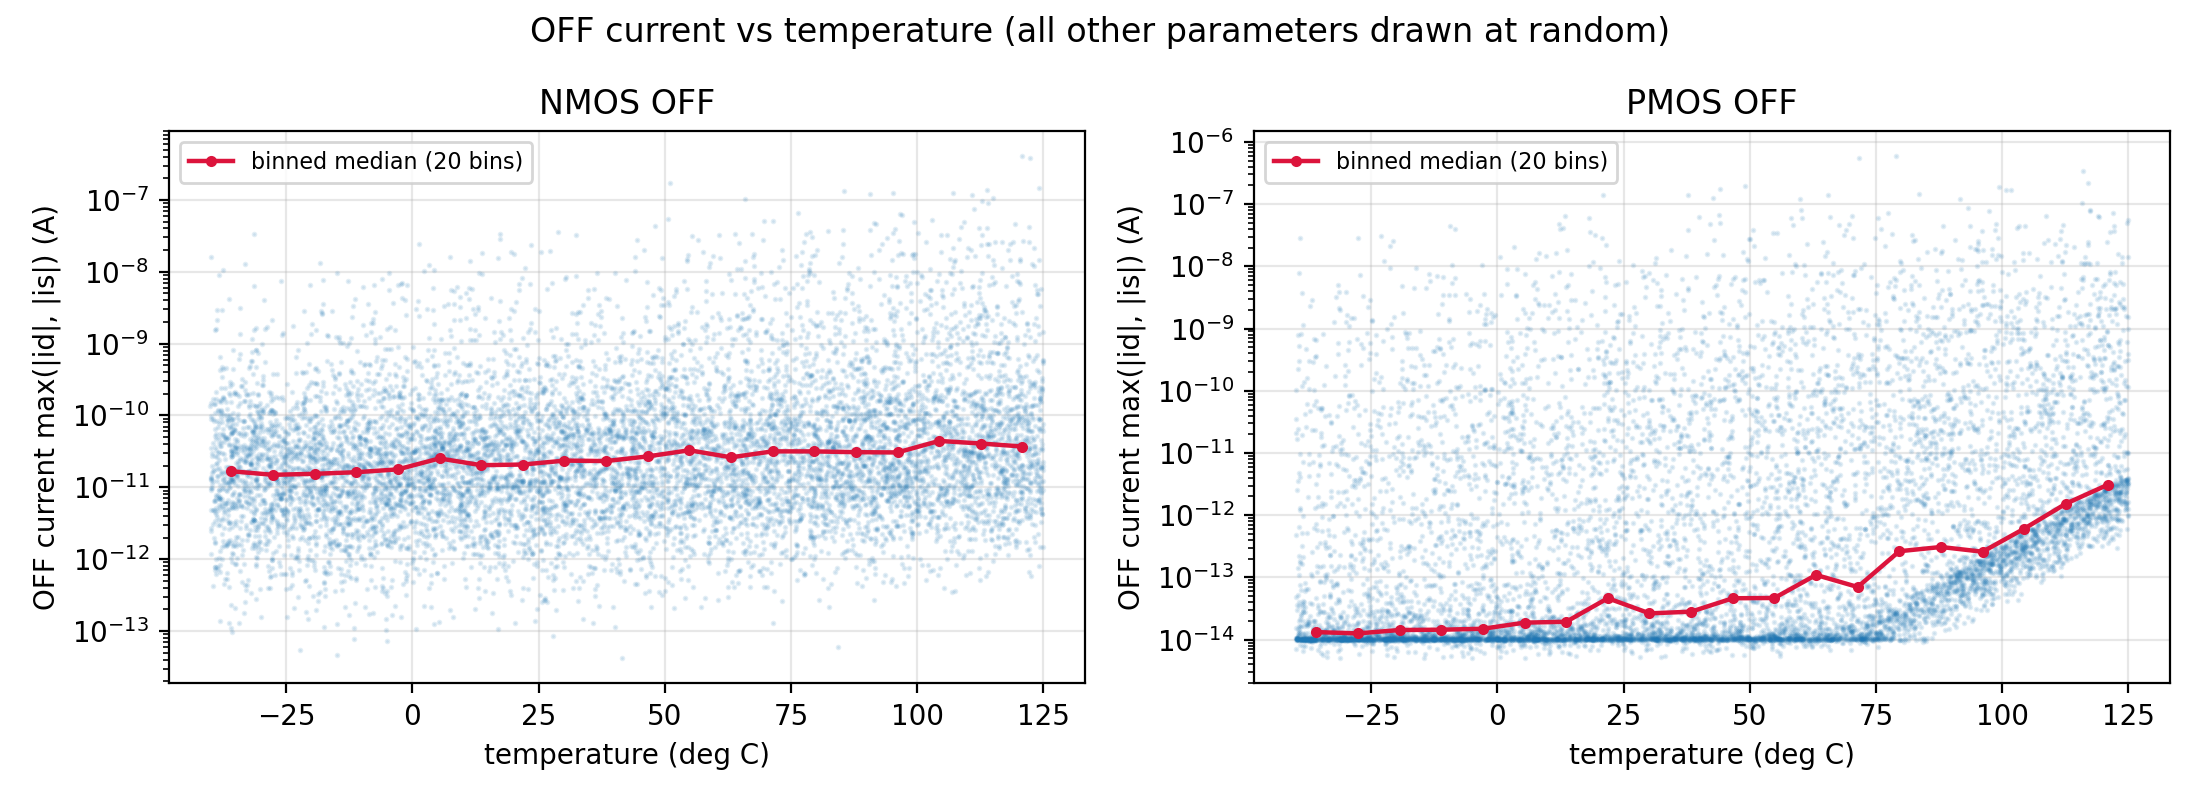
\includegraphics[width=0.49\textwidth]{figures/trend_off_vs_temperature.png}\hfill
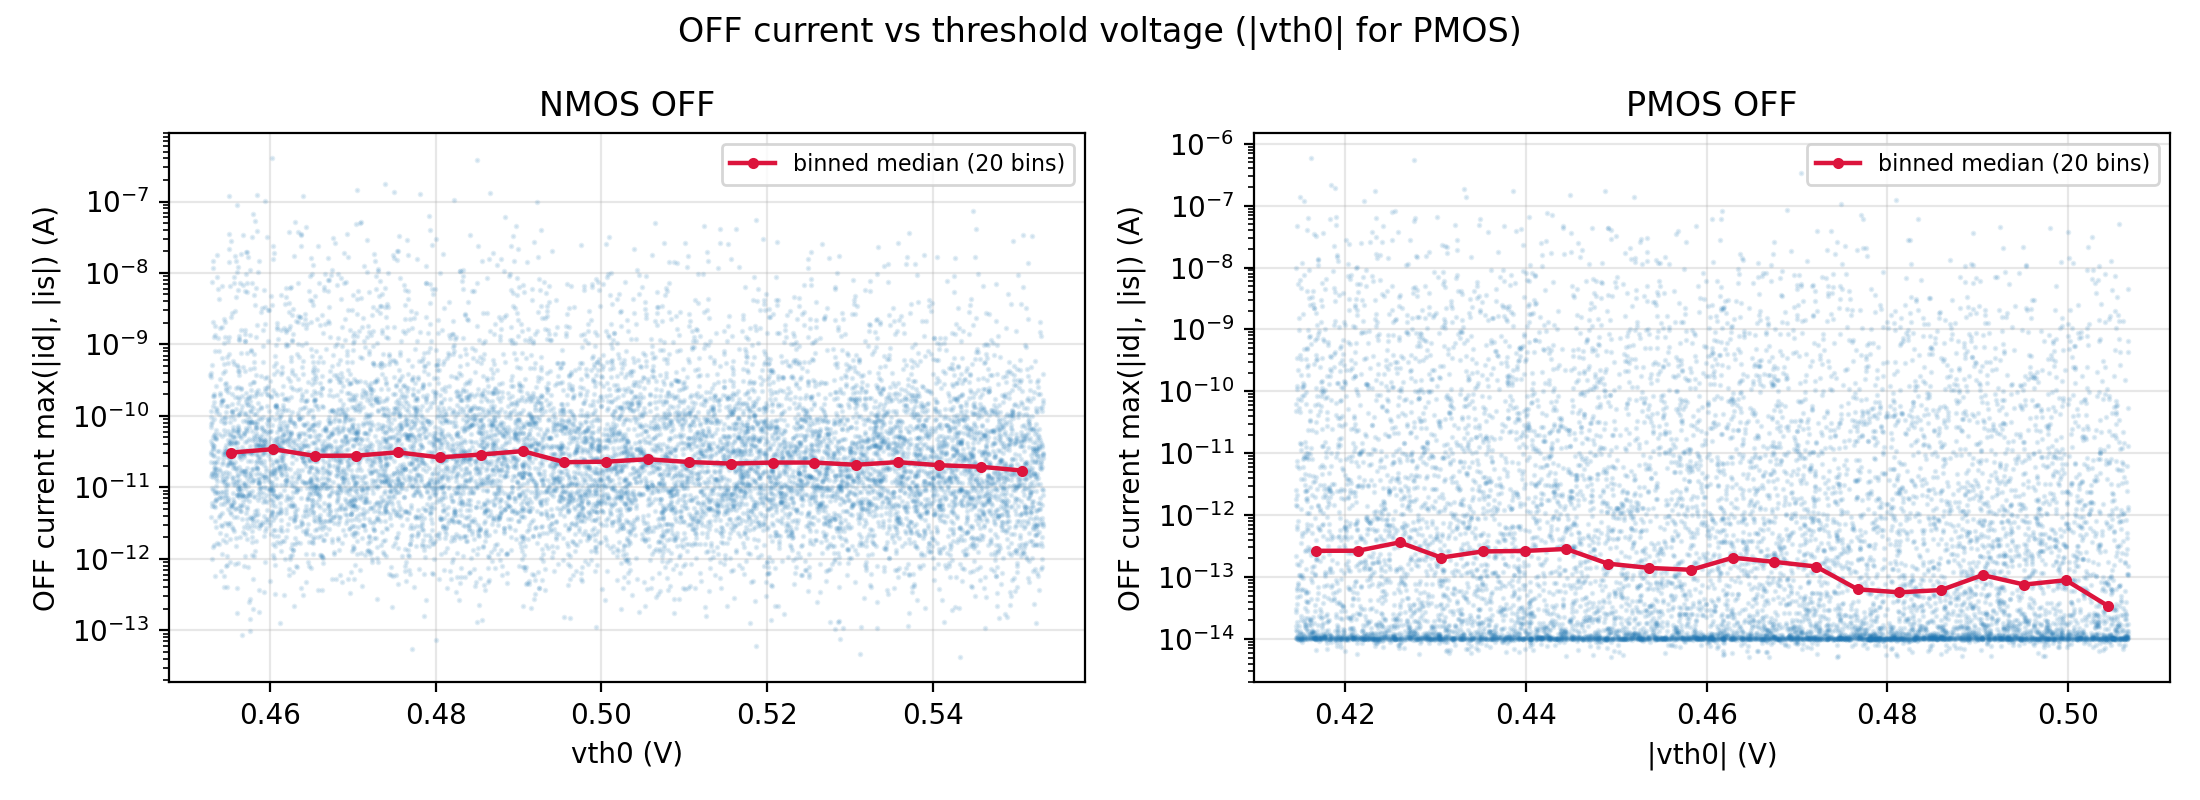
\includegraphics[width=0.49\textwidth]{figures/trend_off_vs_vth0.png}
\caption{OFF current $\max(|i_d|,|i_s|)$ versus temperature (left) and versus $|V_{th0}|$ (right) for NMOS OFF and PMOS OFF; faint points are the 10,000 samples, the red line is the median in 20 bins.}
\label{fig:trend1}
% src: partA_transistor/data_check/trend_off_vs_temperature.png, trend_off_vs_vth0.png
\end{figure*}
\begin{figure*}[t]
\centering
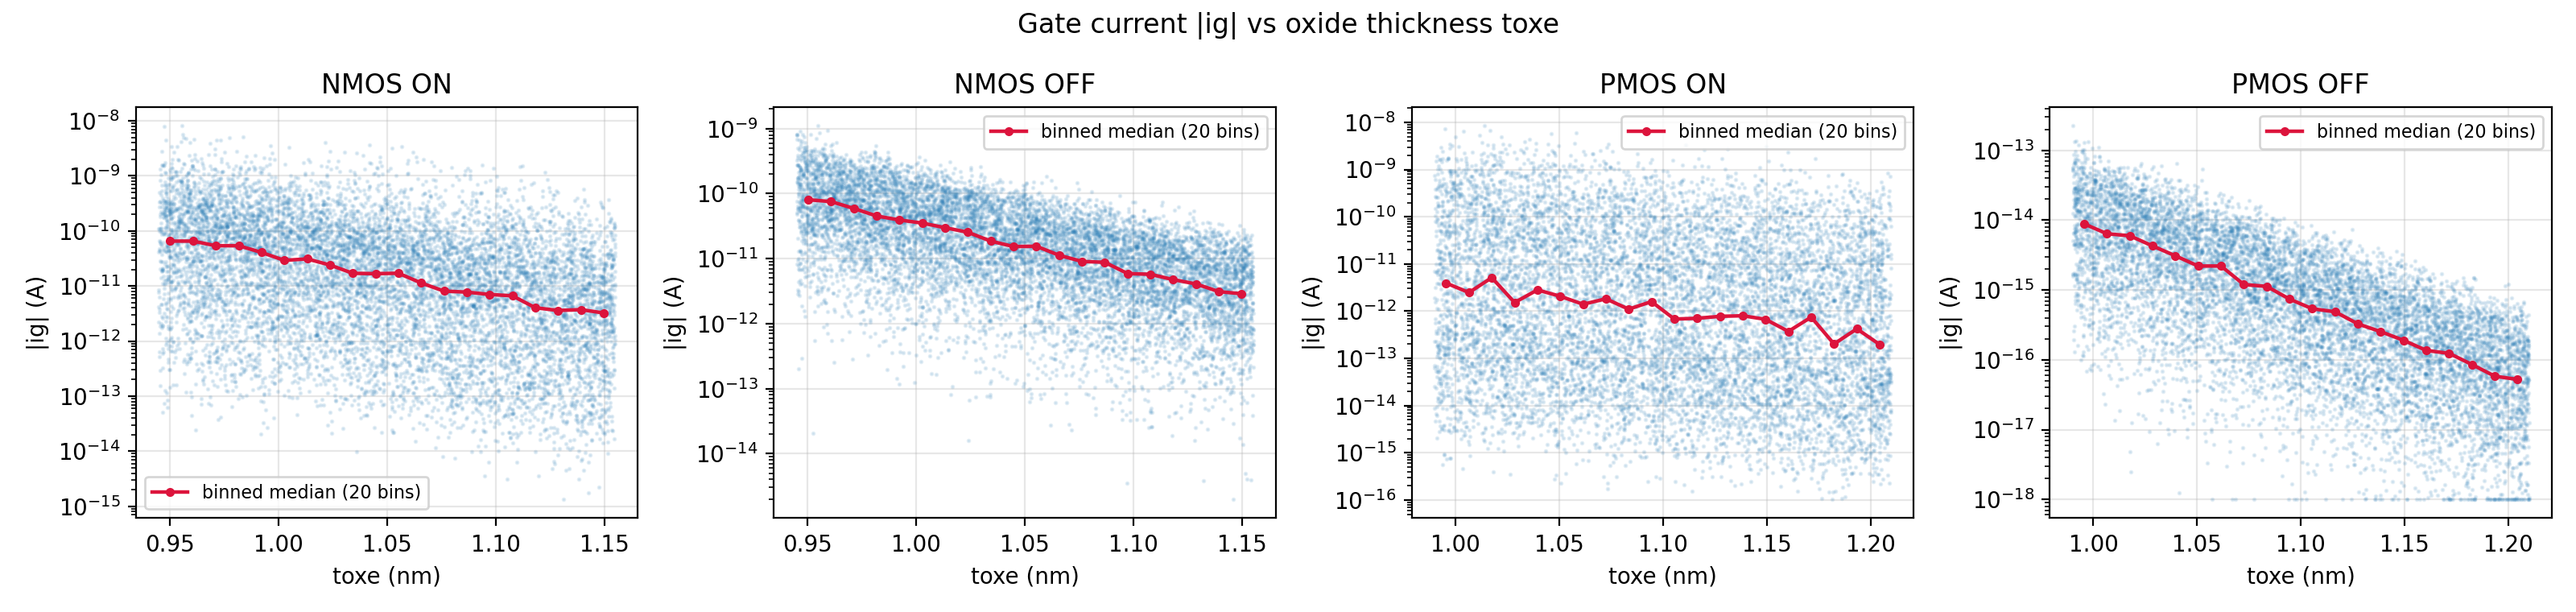
\includegraphics[width=0.9\textwidth]{figures/trend_ig_vs_toxe.png}
\caption{Gate current $|i_g|$ versus oxide thickness for all four cases (tunnelling current: steep fall of the median with toxe).}
\label{fig:trend2}
% src: partA_transistor/data_check/trend_ig_vs_toxe.png
\end{figure*}

\subsection{PMOS OFF gate and body currents}\label{sec:data:readout}
In ngspice a voltage-source branch current is rounded to steps of about \SI{2.22e-16}{\ampere}, while the PMOS OFF gate current is far smaller: 82.51\,\% of the rows have $|i_g|<\SI{5e-15}{\ampere}$. With $i_g=-i(V_g)$ the original PMOS OFF data were mostly rounding noise (1,760 exact zeros, 224 negative values and only 421 distinct values in 10,000 rows). The final netlist therefore reads $i_g$ and $i_b$ from the BSIM4 instance currents, $i_g=-(i_{gs}+i_{gd}+i_{gb}+i_{gcs}+i_{gcd})$ and $i_b=-(i_{bd}+i_{bs})+i_{gb}+i_{sub}+i_{gidl}+i_{gisl}$, which gives 9,977 distinct values and no zeros or negative values; where the source readout is resolvable it agrees to $\num{1.34e-3}$ relative or better. Every terminal still has its own voltage source.
% src: results/analysis/report_numbers/pmos_off_readout_precision.csv, report_data_stats.txt; partA_transistor/netlists/pmos_off_ngspice.cir

\subsection{Output precision, corners and sizing}\label{sec:data:corners}
\texttt{echo} prints six significant digits, so a stored value is rounded by at most $\num{5e-6}$ relative: negligible for currents, but a difference of two six-digit voltages near \SI{1}{\volt} is resolved only to about $10^{-5}$\,\si{\volt} (for NAND2 with inputs 00 the ON-PMOS $|V_{ds}|$ is exactly zero at the stored precision in 130 of 200 rows), which is why the gate leakage is built as in Sec.~\ref{sec:gates:method}.
A corner is one draw of $V_{DD}$, temperature and process parameters; all NMOS of a circuit share one draw and all PMOS another. The 200 corners of Parts~B and~C come from \texttt{rndseed=16} with an identical block and order in all six netlists, so corner~$k$ is the same everywhere (difference 0). Because the random stream behind \texttt{rndseed} depends on the ngspice build, the saved CSV files define the corners and all evaluation reads them.
Gates use $L=\SI{22}{\nano\meter}$ and widths of $2L_{min}$, $4L_{min}$ or $8L_{min}$ inside the training range: inverter PMOS \SI{88}{\nano\meter}, NMOS \SI{44}{\nano\meter}; NAND2 \SI{88}{\nano\meter}; NOR2 PMOS \SI{176}{\nano\meter} (series stack widened), NMOS \SI{44}{\nano\meter}; AND2 and OR2 are the NAND2/NOR2 followed by the inverter. The CLA uses the same gate subcircuits.
% src: validation_checks/digits_check.txt, results/analysis/report_numbers/on_pmos_vds_resolution.csv, validation_checks/b_consistency.txt, partB_gates/netlists/*.cir
